\begin{frame}{Discretización del perfil de obstáculos}
  \begin{columns}[T]
    \begin{column}{0.55\textwidth}
      \begin{block}{Relevamiento por LIDAR}
        El LIDAR del carro releva el \textbf{perfil de obstáculos} $y_{c0}(x,t)$ (pila de
        contenedores, muelle, barco).
      \end{block}

      \begin{block}{Discretización por ancho de contenedor}
        Paso $= W_c = 2.44$ m (contenedor ISO):
        \[
        N_{x_t} = \left\lfloor \frac{x_{t\max}-x_{t\min}}{W_c} \right\rfloor + 1
                = \left\lfloor \frac{80}{2.44} \right\rfloor + 1 = 33
        \]
        Índices $i = 1,\dots,33$.
      \end{block}
    \end{column}
    \begin{column}{0.45\textwidth}
      \centering
      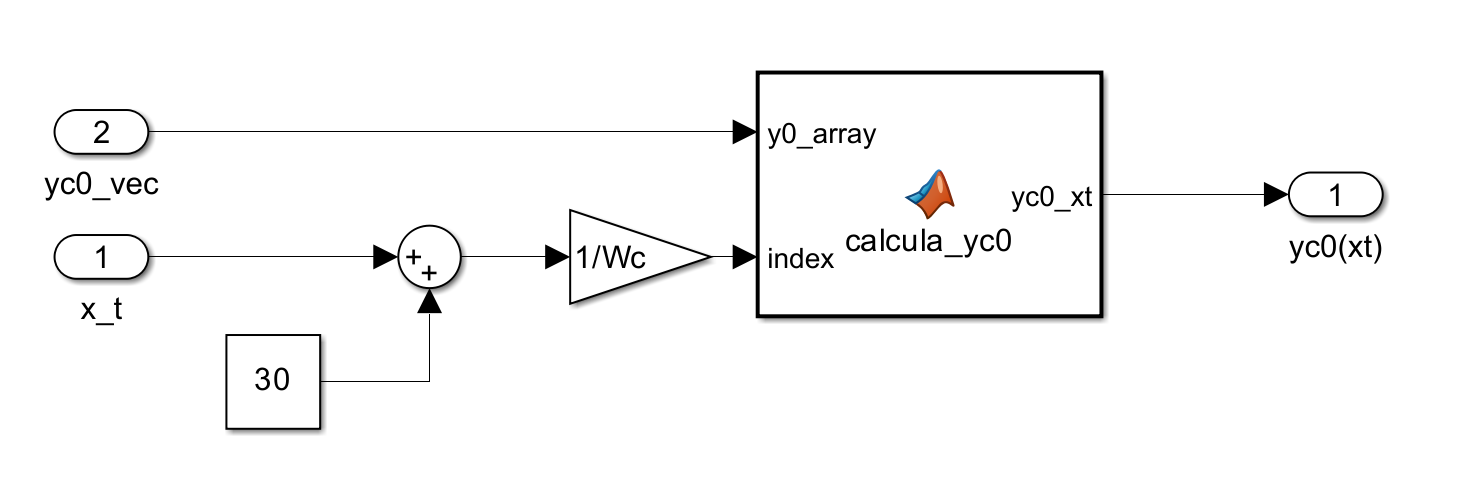
\includegraphics[width=\linewidth]{perfil_obstaculos.png}
    \end{column}
  \end{columns}

  \begin{alertblock}{Vector de perfil $y_{c0\,vec}$}
    Vector de $33$ alturas conocido por el autómata; se \textbf{actualiza} al mover contenedores.
    El modo automático exige el perfil \textbf{escaneado por completo}.
  \end{alertblock}
\end{frame}
